
\begin{DoxyDescription}
\item[Object ]Interesting kind of part of the system, such as a Core, a Cache, a Memory node, etc. The different types detected by hwloc are detailed in the \hyperlink{a00041_gacd37bb612667dc437d66bfb175a8dc55}{hwloc\_\-obj\_\-type\_\-t} enumeration.

They are topologically sorted by CPU set into a tree. 


\item[CPU set ]The set of logical processors (or processing units) logically included in an object (if it makes sense). They are always expressed using physical logical processor numbers (as announced by the OS). They are implemented as the \hyperlink{a00065_gaa3c2bf4c776d603dcebbb61b0c923d84}{hwloc\_\-bitmap\_\-t} opaque structure. hwloc CPU sets are just masks, they do {\itshape not\/} have any relation with an operating system actual binding notion like Linux' cpusets.


\item[Node set ]The set of NUMA memory nodes logically included in an object (if it makes sense). They are always expressed using physical node numbers (as announced by the OS). They are implemented with the \hyperlink{a00065_gaa3c2bf4c776d603dcebbb61b0c923d84}{hwloc\_\-bitmap\_\-t} opaque structure. as bitmaps.


\item[Bitmap ]A possibly-\/infinite set of bits used for describing sets of objects such as CPUs (CPU sets) or memory nodes (Node sets). They are implemented with the \hyperlink{a00065_gaa3c2bf4c776d603dcebbb61b0c923d84}{hwloc\_\-bitmap\_\-t} opaque structure. 


\item[Parent object ]The object logically containing the current object, for example because its CPU set includes the CPU set of the current object.


\item[Ancestor object ]The parent object, or its own parent object, and so on.


\item[Children object(s) ]The object (or objects) contained in the current object because their CPU set is included in the CPU set of the current object.


\item[Arity ]The number of children of an object.


\item[Sibling objects ]Objects which have the same parent. They usually have the same type (and hence are cousins, as well), but they may not if the topology is asymmetric.


\item[Sibling rank ]Index to uniquely identify objects which have the same parent, and is always in the range \mbox{[}0, parent\_\-arity).


\item[Cousin objects ]Objects of the same type (and depth) as the current object, even if they do not have the same parent.


\item[Level ]Set of objects of the same type and depth. All these objects are cousins.


\item[Depth ]Nesting level in the object tree, starting from the root object. If the topology is symmetric, the depth of a child is equal to the parent depth plus one, and an object depth is also equal to the number of parent/child links between the root object and the given object. If the topology is asymmetric, the difference between some parent and child depths may be larger than one when some intermediate levels (for instance caches) are missing in only some parts of the machine. 


\item[OS or physical index ]The index that the operating system (OS) uses to identify the object. This may be completely arbitrary, non-\/unique, non-\/contiguous, not representative of logical proximity, and may depend on the BIOS configuration. That is why hwloc almost never uses them, only in the default lstopo output ({\ttfamily P::x}) and cpuset masks.


\item[Logical index ]Index to uniquely identify objects of the same type and depth, automatically computed by hwloc according to the topology. It expresses logical proximity in a generic way, i.e. objects which have adjacent logical indexes are adjacent in the topology. That is why hwloc almost always uses it in its API, since it expresses logical proximity. They can be shown (as {\ttfamily L::x}) by {\ttfamily lstopo} thanks to the {\ttfamily -\/l} option. This index is always linear and in the range \mbox{[}0, num\_\-objs\_\-same\_\-type\_\-same\_\-level-\/1\mbox{]}. Think of it as ``cousin rank.'' The ordering is based on topology first, and then on OS CPU numbers, so it is stable across everything except firmware CPU renumbering. \char`\"{}Logical index\char`\"{} should not be confused with \char`\"{}Logical processor\char`\"{}. A \char`\"{}Logical
  processor\char`\"{} (which in hwloc we rather call \char`\"{}processing unit\char`\"{} to avoid the confusion) has both a physical index (as chosen arbitrarily by BIOS/OS) and a logical index (as computed according to logical proximity by hwloc). 


\item[Logical processor ]
\item[Processing unit ]The smallest processing element that can be represented by a hwloc object. It may be a single-\/core processor, a core of a multicore processor, or a single thread in SMT processor. \char`\"{}Logical processor\char`\"{} should not be confused with \char`\"{}Logical index of a
  processor\char`\"{}. \char`\"{}Logical processor\char`\"{} is only one of the names which can be found in various documentations to designate a processing unit. 


\end{DoxyDescription}

The following diagram can help to understand the vocabulary of the relationships by showing the example of a machine with two dual core sockets (with no hardware threads); thus, a topology with 4 levels. Each box with rounded corner corresponds to one hwloc\_\-obj\_\-t, containing the values of the different integer fields (depth, logical\_\-index, etc.), and arrows show to which other hwloc\_\-obj\_\-t pointers point to (first\_\-child, parent, etc.). The L2 cache of the last core is intentionally missing to show how asymmetric topologies are handled.

 
\begin{DoxyImageNoCaption}
  \mbox{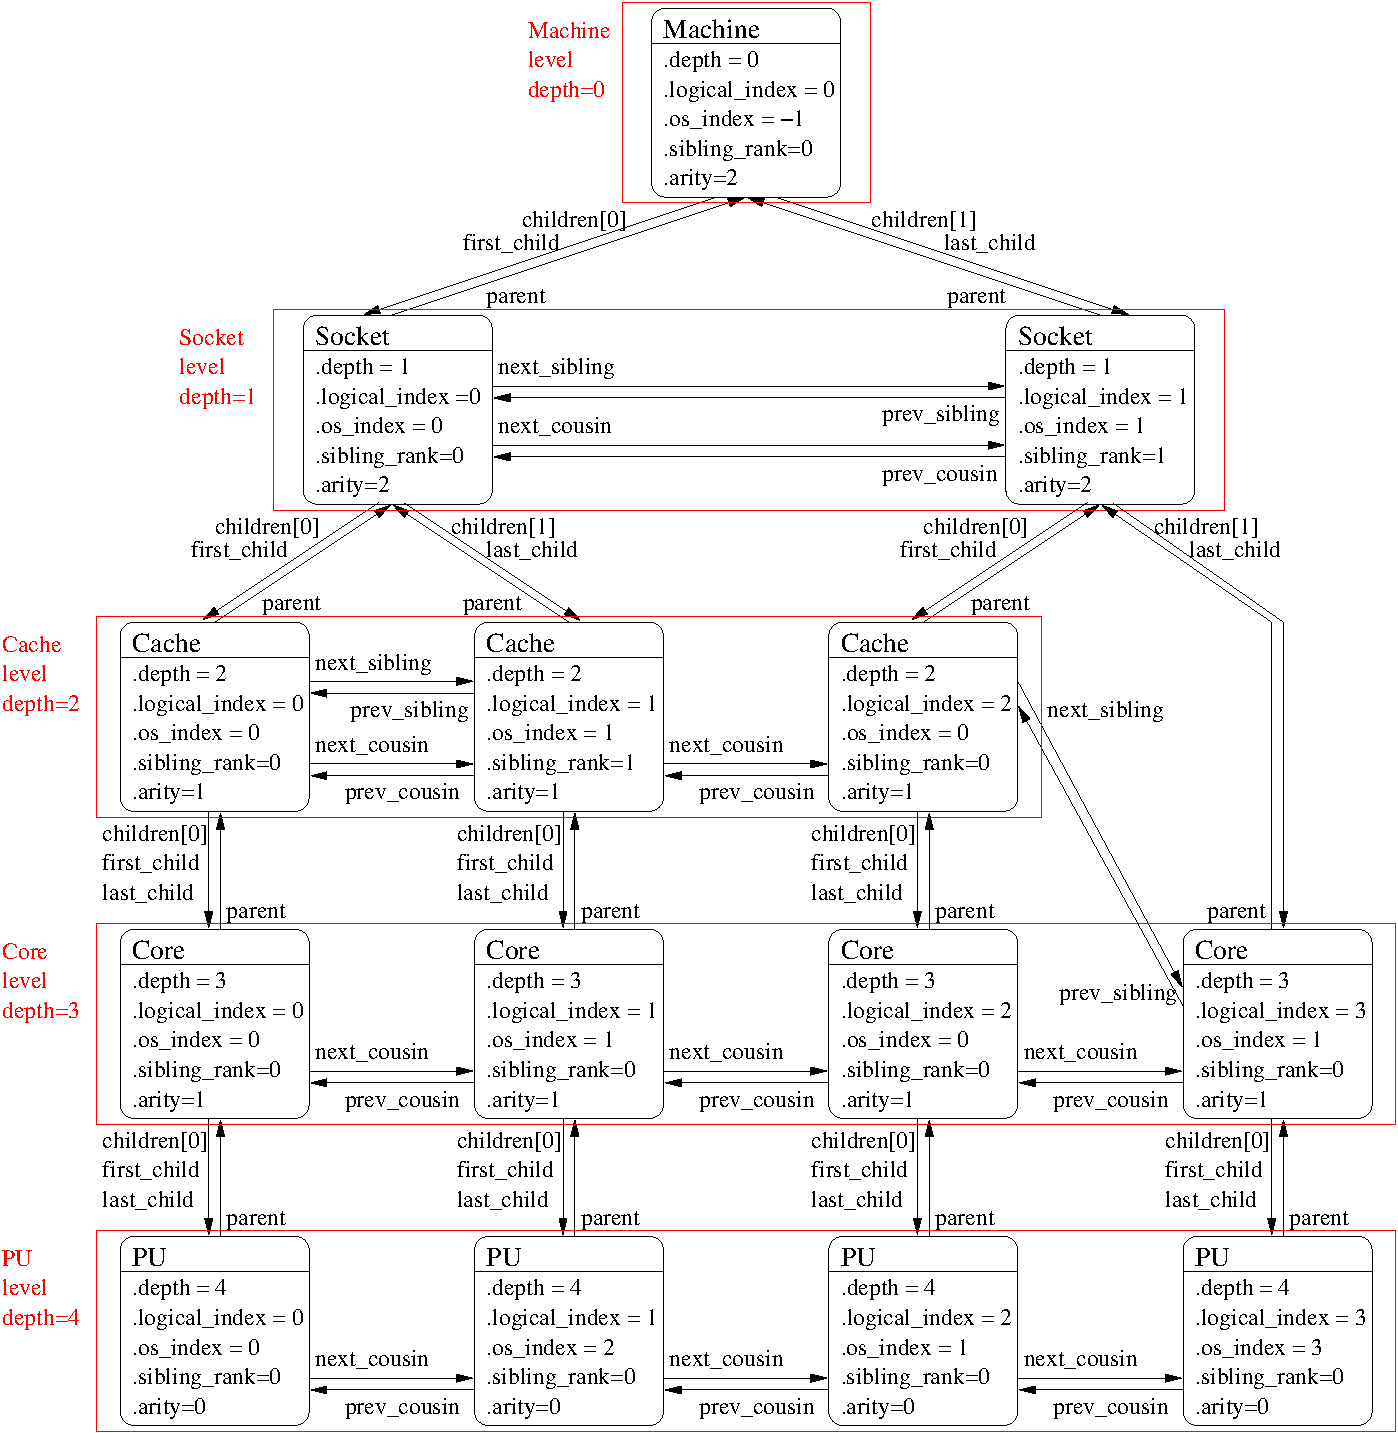
\includegraphics[width=\textwidth]{diagram}}
\end{DoxyImageNoCaption}


It should be noted that for PU objects, the logical index -\/-\/ as computed linearly by hwloc -\/-\/ is not the same as the OS index.

See also \hyperlink{a00011_faq_asymmetric}{What happens if my topology is asymmetric?} for more details. 